% Note: this need to be compiled twice! 
\documentclass[11pt,twocolumn,landscape,a4paper,notitlepage]{article}

% Packages
\usepackage{calc}			% for length arithmetic.
\usepackage[twocolumn, top=1.0cm, bottom=1.0cm, left=1.0cm, right=1.0cm, voffset=0cm, hoffset=0cm, headsep=0.2cm, headheight=13.6pt, footskip=\headsep + \headheight, columnsep=1.25cm]{geometry}
\usepackage{babel}
\usepackage{listings} 				% for code snippets.
\usepackage{fancyhdr}				% for headers and footers.
\usepackage{etoolbox}				% for the \maketitle hack.
\usepackage{array}					% for table column specifications.
\usepackage{graphicx}				% for table resize.
\usepackage{booktabs}				% for tables.
\usepackage{xtab}					% for multiple pages tables.
\usepackage[hidelinks]{hyperref}	% for click-able toc
\usepackage{amsmath}
\usepackage{graphicx}
\usepackage{ragged2e}
\usepackage{xcolor}

% Dibujar grafos
\usepackage{tikz} 

\lstnewenvironment{code}
    {%\lstset{	numbers=none, frame=lines, basicstyle=\small\ttfamily, }%
    \csname lst@SetFirstLabel\endcsname}
    {\csname lst@SaveFirstLabel\endcsname}
% We create some new table columns types.
\newcolumntype{L}[1]{>{\raggedright\let\newline\\\arraybackslash\hspace{0pt}}m{#1-2\tabcolsep- 1.25\arrayrulewidth}}
\newcolumntype{C}[1]{>{\centering\let\newline\\\arraybackslash\hspace{0pt}}m{#1-2\tabcolsep- 1.25\arrayrulewidth}}
\newcolumntype{R}[1]{>{\raggedleft\let\newline\\\arraybackslash\hspace{0pt}}m{#1-2\tabcolsep- 1.25\arrayrulewidth}}

% We make visible heder's and footer's ruler.
\renewcommand{\headrulewidth}{0.5pt}
\renewcommand{\footrulewidth}{0.5pt}
\renewcommand{\columnseprule}{0.5pt}

% To display the footer and header on the first page.
\fancypagestyle{plain}
{
	\fancyhf{}
	\rhead{piashi piashii}
	\lhead{UTN FRRO - hola}
	\rfoot{P\'agina \thepage}
}
\pagestyle{plain}

% and for the rest of the pages.
\fancyhf{}
\rhead{\leftmark}
\lhead{UTN FRRO - hola}
\rfoot{P\'agina \thepage}

% We use Courier font to make bold keywords possible.
% \renewcommand{\ttdefault}{pcr}

\usepackage{xcolor}
\definecolor{commentgreen}{RGB}{2,112,10}

% Listing code style
\lstdefinestyle{codestyle}{
	basicstyle=\scriptsize\ttfamily,
    keywordstyle=\bfseries,
    emph={int,char,double,float,unsigned,void,bool},
    emphstyle=\bfseries,
    breakatwhitespace=false,
    breaklines=true,
    captionpos=b,
    keepspaces=false,
    numbers=left,
    numberstyle=\tiny\ttfamily,
    numbersep=5pt,
    frame=single,
    framesep=3pt,
    showspaces=false,
    showstringspaces=false,
    showtabs=false,
    tabsize=2,
    commentstyle=\color{commentgreen}, % comment color
    keywordstyle=\color{blue}, % keyword color
    stringstyle=\color{red} % string color
}
\lstset{style=codestyle}

% To dislpay the title on one column 
\makeatletter
% Remove the brackets so LaTeX sees \twocolumn\@maketitle
\patchcmd{\maketitle}{[\@maketitle]}{\@maketitle}{}{}
% Remove the vertical shift from the title 
\patchcmd{\@maketitle}{\null\vskip2em\begin{center}}{\vspace*{0pt}\nointerlineskip\begingroup\centering}{}{}
% In the final part we must remove \end{center}
\patchcmd{\@maketitle}{\end{center}\par}{\par\endgroup}{}{}
\makeatother


% Information
\author{UTN FRRO - HOLA}
\title{Notebook}
\date{2024}


\begin{document}
\maketitle
\centering{
\includegraphics[width=12cm]{portada}}\newpage
\tableofcontents
\newpage

% Here we include each section of this notebook from external files.
\newpage
\section{Basics}

\subsection{Template}
\lstinputlisting[language=C++]{secciones/basics/template.cpp}

\subsection{Compilation}
\begin{lstlisting}
g++ -DEBUG <ej>.cpp -o a && time ./a
\end{lstlisting}
\newpage

\section{Math}

\subsection{Identidades}
{
$\sum_{i=0}^n\binom{n}{i}=2^n$

$\sum_{i=0}^n i\binom{n}{i}=n*2^{n-1}$

$\sum_{i=m}^n i = \frac{n(n+1)}{2} - \frac{m(m-1)}{2} = \frac{(n+1-m)(n+m)}{2}$

$\sum_{i=0}^n i = \sum_{i=1}^n i = \frac{n(n+1)}{2}$

$\sum_{i=0}^n i^2 = \frac{n(n+1)(2n+1)}{6} = \frac{n^3}{3} + \frac{n^2}{2} + \frac{n}{6}$

$\sum_{i=0}^n i(i-1) = \frac{8}{6}(\frac{n}{2})(\frac{n}{2}+1)(n+1)$ (doubles) $\rightarrow$ Sino ver caso impar y par

$\sum_{i=0}^n i^3 = \left(\frac{n(n+1)}{2}\right)^2 = \frac{n^4}{4} + \frac{n^3}{2} + \frac{n^2}{4} = \left[\sum_{i=1}^n i\right]^2$

$\sum_{i=0}^n i^4 = \frac{n(n+1)(2n+1)(3n^2+3n-1)}{30} = \frac{n^5}{5} + \frac{n^4}{2} + \frac{n^3}{3} - \frac{n}{30}$

$\sum_{i=0}^n i^p = \frac{(n+1)^{p+1}}{p+1} + \sum_{k=1}^p\frac{B_k}{p-k+1}{p\choose k}(n+1)^{p-k+1}$
}%

\subsection{Tablas y cotas (Primos, Divisores, Factoriales, etc)}
%\subsubsection{
\paragraph{Factoriales} \ \\
\begin{tabular}{l|l}
0! =	1             & 11! = 39.916.800  \\
1! =	1             & 12! =	479.001.600	($\in \mathtt{int}$)\\
2! =	2             & 13! =	6.227.020.800	\\
3! =	6             & 14! =	87.178.291.200	\\
4! =	24            & 15! =	1.307.674.368.000	\\
5! =	120   	      & 16! =	20.922.789.888.000	\\
6! =	720           & 17! =	355.687.428.096.000	\\
7! =	5.040	      & 18! =	6.402.373.705.728.000	\\
8! =	40.320	      & 19! =	121.645.100.408.832.000	\\
9! =	362.880       & 20! =	2.432.902.008.176.640.000	($\in \mathtt{tint}$) \\
10! =	3.628.800     & 21! =	51.090.942.171.709.400.000
\end{tabular}

%\subsubsection{
\paragraph{Primos} \ \\
2 3 5 7 11 13 17 19 23 29
31 37 41 43 47 53 59 61 67 71
73 79 83 89 97 101 103 107 109 113
127 131 137 139 149 151 157 163 167 173
179 181 191 193 197 199 211 223 227 229
233 239 241 251 257 263 269 271 277 281
283 293 307 311 313 317 331 337 347 349
353 359 367 373 379 383 389 397 401 409
419 421 431 433 439 443 449 457 461 463
467 479 487 491 499 503 509 521 523 541
547 557 563 569 571 577 587 593 599 601
607 613 617 619 631 641 643 647 653 659
661 673 677 683 691 701 709 719 727 733
739 743 751 757 761 769 773 787 797 809
811 821 823 827 829 839 853 857 859 863
877 881 883 887 907 911 919 929 937 941
947 953 967 971 977 983 991 997 1009 1013
1019 1021 1031 1033 1039 1049 1051 1061 1063 1069
1087 1091 1093 1097 1103 1109 1117 1123 1129 1151
1153 1163 1171 1181 1187 1193 1201 1213 1217 1223
1229 1231 1237 1249 1259 1277 1279 1283 1289 1291
1297 1301 1303 1307 1319 1321 1327 1361 1367 1373
1381 1399 1409 1423 1427 1429 1433 1439 1447 1451
1453 1459 1471 1481 1483 1487 1489 1493 1499 1511
1523 1531 1543 1549 1553 1559 1567 1571 1579 1583
1597 1601 1607 1609 1613 1619 1621 1627 1637 1657
1663 1667 1669 1693 1697 1699 1709 1721 1723 1733
1741 1747 1753 1759 1777 1783 1787 1789 1801 1811
1823 1831 1847 1861 1867 1871 1873 1877 1879 1889
1901 1907 1913 1931 1933 1949 1951 1973 1979 1987
1993 1997 1999 2003 2011 2017 2027 2029 2039 2053
2063 2069 2081
\paragraph{Primos cercanos a $10^n$}\ \\
9941 9949 9967 9973 10007 10009 10037 10039 10061 10067 10069 10079\\
99961 99971 99989 99991 100003 100019 100043 100049 100057 100069\\
999959 999961 999979 999983 1000003 1000033 1000037 1000039\\
9999943 9999971 9999973 9999991 10000019 10000079 10000103 10000121\\
99999941 99999959 99999971 99999989 100000007 100000037 100000039 100000049\\
999999893 999999929 999999937 1000000007 1000000009 1000000021 1000000033
 
\paragraph{Cantidad de primos menores que $10^n$}\ \\
$\pi(10^1)$ = 4 ;
$\pi(10^2)$ = 25 ;
$\pi(10^3)$ = 168 ;
$\pi(10^4)$ = 1229 ;
$\pi(10^5)$ = 9592 \\
$\pi(10^6)$ = 78.498 ;
$\pi(10^7)$ = 664.579 ;
$\pi(10^8)$ = 5.761.455 ;
$\pi(10^9)$ = 50.847.534 \\
$\pi(10^{10})$ = 455.052,511 ;
$\pi(10^{11})$ = 4.118.054.813 ;
$\pi(10^{12})$ = 37.607.912.018% ;
%
% Fuente: http://primes.utm.edu/howmany.shtml#table
%
%
\newpage
\subsection{Reglas de divisibilidad}
\begin{center}
\tablefirsthead{\hline \textbf{Nro} & \textbf{Regla} & \textbf{Ejemplo} \\ \hline}
\tablehead{\hline \multicolumn{3}{|c|}{\tiny Contin\'ua} \\ \hline \textbf{Nro} & \textbf{Regla} & \textbf{Ejemplo} \\ }
% \tabletail{\hline}
% \tablelasttail{\hline}
\footnotesize
{
  \begin{xtabular}{|L{.1\columnwidth}|C{.4\columnwidth}|L{.4\columnwidth}|}
    1 & Todos los números & 5: porque si divides 5:1=5 y ese número es un múltiplo o divisor de cualquier número. \\ \hline
    2 & El número termina en una cifra par. & 378: porque la última cifra (8) es par. \\ \hline
    3 & La suma de sus cifras es un múltiplo de 3. & 480: porque 4+8+0=12 es múltiplo de 3. \\ \hline
    4 & Sus últimos dos dígitos son 0 o un múltiplo de 4. & 300 y 516 son divisibles entre 4 porque terminan en 00 y en 16, respectivamente, siendo este último un múltiplo de 4 (16=4*4). \\ \hline
    5 & La última cifra es 0 o 5. & 485: porque termina en 5. \\ \hline
    7 & Un número es divisible entre 7 cuando, al separar la última cifra de la derecha, multiplicarla por 2 y restarla de las cifras restantes la diferencia es igual a 0 o es un múltiplo de 7. Otro sistema: Si la suma de la multiplicación de los números por la serie 2,3,1,-2,-3,-1... da 0 o un múltiplo de 7. & 34349: separamos el 9, y lo duplicamos (18), entonces 3434-18=3416. Repetimos el proceso separando el 6 (341'6) y duplicándolo (12), entonces 341-12=329, y de nuevo, 32'9, 9*2=18, entonces 32-18=14; por lo tanto, 34349 es divisible entre 7 porque 14 es múltiplo de 7. Ejemplo método 2: 34349: [(2*3)+(3*4)+(1*3)-(2*4)-(3*9)]= 6+12+3-8-27 = -14.8 \\ \hline
    8 & Para saber si un número es divisible entre 8 hay que comprobar que sus tres últimas cifras sean divisibles entre 8. Si sus tres últimas cifras son divisibles entre 8 entonces el número también es divisible entre 8. & Ejemplo: El número 571.328 es divisible por 8 ya que sus últimas tres cifras (328) son divisibles por 8 (32 = 8*4 y 8 = 8*1). Realizando la división comprobamos que 571.328 : 8 = 71.416 \\ \hline
    9 & Un número es divisible por 9 cuando al sumar todas sus cifras el resultado es múltiplo de 9. & 504: sumamos 5+0+4=9 y como 9 es múltiplo de 9 504 es divisible por 9 5346: sumamos 5+3+4+6=18 y como 18 es múltiplo de 9, 5346 es divisible por 9. \\ \hline
    10 & La última cifra es 0. & 4680: porque termina en 0 \\ \hline
    11 & Sumando las cifras (del número) en posición impar por un lado y las de posición par por otro. Luego se resta el resultado de ambas sumas obtenidas. Si el resultado es cero o un múltiplo de 11, el número es divisible entre este. Si el número tiene solo dos cifras y estas son iguales será múltiplo de 11. & 42702: 4+7+2=13 · 2+0=2 · 13-2=11 → 42702 es múltiplo de 11. 66: porque las dos cifras son iguales. Entonces 66 es múltiplo de 11. \\ \hline
    13 & Un número es divisible entre 13 cuando, al separar la última cifra de la derecha, multiplicarla por 9 y restarla de las cifras restantes la diferencia es igual a 0 o es un múltiplo de 13 & 3822: separamos el último dos (382'2) y lo multiplicamos por 9, 2×9=18, entonces 382-18=364. Repetimos el proceso separando el 4 (36'4) y multiplicándolo por 9, 4×9=36, entonces 36-36=0; por lo tanto, 3822 es divisible entre 13. \\ \hline
    17 & Un número es divisible entre 17 cuando, al separar la última cifra de la derecha, multiplicarla por 5 y restarla de las cifras restantes la diferencia es igual a 0 o es un múltiplo de 17 & 2142: porque 214'2, 2*5=10, entonces 214-10=204, de nuevo, 20'4, 4*5=20, entonces 20-20=0; por lo tanto, 2142 es divisible entre 17. \\ \hline
    19 & Un número es divisible entre 19 si al separar la cifra de las unidades, multiplicarla por 2 y sumar a las cifras restantes el resultado es múltiplo de 19. & 3401: separamos el 1, lo doblamos (2) y sumamos 340+2= 342, ahora separamos el 2, lo doblamos (4) y sumamos 34+4=38 que es múltiplo de 19, luego 3401 también lo es. \\ \hline
    20 & Un número es divisible entre 20 si sus dos últimas cifras son ceros o múltiplos de 20. Cualquier número par que tenga uno o más ceros a la derecha, es múltiplo de 20. & 57860: Sus 2 últimas cifras son 60 (Que es divisible entre 20), por lo tanto 57860 es divisible entre 20. \\ \hline
    23 & Un número es divisible entre 23 si al separar la cifra de las unidades, multiplicar por 7 y sumar las cifras restantes el resultado es múltiplo de 23. & 253: separamos el 3, lo multiplicamos por 7 y sumamos 25+21= 46, 46 es múltiplo de 23 así que es divisible entre 23. \\ \hline
    25 & Un número es divisible entre 25 si sus dos últimas cifras son 00, o en múltiplo de 25 (25,50,75,...) & 650: Es múltiplo de 25 por lo cual es divisible. 400 también será divisible entre 25. \\ \hline
    29 & Un número es divisible entre 29 cuando, al separar la última cifra de la derecha, multiplicarla por 3 y restarla de las cifras restantes la diferencia es igual a 0 o es un múltiplo de 29 & 2436: separamos el 6 (243'6) y lo multiplicamos por 3, 6×3=18, entonces 243-18=225. Repetimos el proceso separando el 5 (22'5) y multiplicándolo por 3, 5×3=15, entonces 22-15=7, que no es divisible entre 29. \\ \hline
  \end{xtabular}
}
\end{center}


\subsection{Coprimos}
Son aquellos números enteros \(a\) y \(b\) cuyo único factor en común que tienen es 1. Equivalentemente son coprimos, si, y solo si, su máximo común divisor (MCD) es igual a 1. Dos números coprimos no tienen por qué ser primos absolutos de forma individual. 14 y 15 son compuestos, sin embargo son coprimos, pues: 
\( gcd(14,15) = 1\)

\subsection{Primos}
\lstinputlisting[language=C++]{secciones/math/primos.cpp}

\subsection{Combinatoria}
\lstinputlisting[language=C++]{secciones/math/combinatoria.cpp}

\newpage

\newpage
\section{Estructuras}

\subsection{vector}
\begin{center}
    \begin{tabular}{||l|l|l||}
        \hline
        \textbf{Función}          & \textbf{Explicación}                              & \textbf{O} \\ \hline
        (constructor)             & Construct vector                                  & O(n)                 \\ \hline
        (destructor)              & Vector destructor                                 & O(n)                 \\ \hline
        operator=                 & Assign content                                    & O(n)                 \\ \hline
        begin                     & Return iterator to beginning                      & O(1)                 \\ \hline
        end                       & Return iterator to end                            & O(1)                 \\ \hline
        rbegin                    & Return reverse iterator to reverse beginning      & O(1)                 \\ \hline
        rend                      & Return reverse iterator to reverse end            & O(1)                 \\ \hline
        cbegin                    & Return const\_iterator to beginning               & O(1)                 \\ \hline
        cend                      & Return const\_iterator to end                     & O(1)                 \\ \hline
        crbegin                   & Return const\_reverse\_iterator to reverse beginning  & O(1)             \\ \hline
        crend                     & Return const\_reverse\_iterator to reverse end    & O(1)                 \\ \hline
        size                      & Return size                                       & O(1)                 \\ \hline
        resize                    & Change size                                       & O(n)                 \\ \hline
        empty                     & Test whether vector is empty                      & O(1)                 \\ \hline
        operator[]                & Access element                                    & O(1)                 \\ \hline
        at                        & Access element                                    & O(1)                 \\ \hline
        front                     & Access first element                              & O(1)                 \\ \hline
        back                      & Access last element                               & O(1)                 \\ \hline
        assign                    & Assign vector content                             & O(n)                 \\ \hline
        push\_back                & Add element at the end                            & O(1) \\ \hline
        pop\_back                 & Delete last element                               & O(1)                 \\ \hline
        insert                    & Insert elements                                   & O(n)                 \\ \hline
        erase                     & Erase elements                                    & O(n)                 \\ \hline
        swap                      & Swap content                                      & O(1)                 \\ \hline
        clear                     & Clear content                                     & O(n)                 \\ \hline
        emplace                   & Construct and insert element                      & O(1) \\ \hline
        emplace\_back             & Construct and insert element at the end           & O(1) \\ \hline
    \end{tabular}
\label{tab:vector_member_functions_complexity}
\end{center}

\newpage
\subsubsection{emplace}
\begin{lstlisting}[language=C++]
vector<int> myvector = {10,20,30};

auto it = myvector.emplace ( myvector.begin()+1, 100 );
myvector.emplace ( it, 200 );
myvector.emplace ( myvector.end(), 300 );

for (auto& x: myvector)
    cout << ' ' << x;
// 10 200 100 20 30 300
\end{lstlisting}

\subsubsection{resize}
Resizes the container so that it contains n elements. \\
\lstinline[language=C++]{void resize (size_type n, const value_type& val);}
\begin{lstlisting}[language=C++]
vector<int> myvector;
for (int i=1; i<10; i++) myvector.push_back(i);

myvector.resize(5);
myvector.resize(8, 100);
myvector.resize(12);

for (int i=0;i<myvector.size();i++)
    cout << ' ' << myvector[i];
//  1 2 3 4 5 100 100 100 0 0 0 0
\end{lstlisting}

\subsubsection{assign}
Assigns new contents to the vector, replacing its current contents, and modifying its size accordingly. \\
\lstinline[language=C++]{void assign (size_type n, const value_type& val);

\begin{lstlisting}[language=C++]
vector<int> first;
vector<int> second;
vector<int> third;

first.assign (7,100);             // 7 ints with a value of 100

vector<int>::iterator it;
it=first.begin()+1;

second.assign (it,first.end()-1); // the 5 central values of first

int myints[] = {1776,7,4};
third.assign (myints,myints+3);   // assigning from array.

first.size() // -> 7
second.size() // -> 5
third.size()) // -> 3

\end{lstlisting}



\subsection{unordered set}
\begin{center}
    \begin{tabular}{||l|l|l||}
        \hline
        \textbf{Función}         & \textbf{Explicación}                               & \textbf{O} \\ \hline
        (constructor)            & Construct unordered\_set                          & -    \\ \hline
        (destructor)             & Destroy unordered\_set                            & -    \\ \hline
        operator=                & Assign content                                    & O(n) \\ \hline
        empty                    & Test whether container is empty                   & O(1) \\ \hline
        size                     & Return container size                             & O(1) \\ \hline
        max\_size                & Return maximum size                               & O(1) \\ \hline
        begin                    & Return iterator to beginning                      & O(1) \\ \hline
        end                      & Return iterator to end                            & O(1) \\ \hline
        find                     & Get iterator to element                           & O(n) \\ \hline
        count                    & Count elements with a specific key                & O(n) \\
                                 & Returns 0 or 1                                    & \\ \hline
        equal\_range             & Get range of elements with a specific key         & O(n) \\ \hline
        emplace                  & Construct and insert element                      & O(n) \\ \hline
        emplace\_hint            & Construct and insert element with hint            & O(n) \\ \hline
        insert                   & Insert elements                                   & O(n) \\ \hline
        erase                    & Erase elements                                    & O(n) \\ \hline
        clear                    & Clear content                                     & O(n) \\ \hline
        swap                     & Swap content                                      & O(1) \\ \hline
        reserve                  & Request a capacity change                         & O(n) \\ \hline
        key\_eq                  & Get key equivalence predicate                     & O(1) \\ \hline
    \end{tabular}
    \label{tab:set_member_functions_complexity}
\end{center}
\newpage

\begin{lstlisting}[language=C++]
unordered_set<int> s;
s.insert(3);
s.insert(5);
s.erase(3);
s.count(3); // -> 0
s.count(5); // -> 1
\end{lstlisting}


\subsection{Iterators}
\begin{lstlisting}[language=C++]
sort(v.begin(), v.end());
reverse(v.begin(), v.end());
random_shuffle(v.begin(), v.end());

sort(v.begin(), v.end(), sortbysec);
\end{lstlisting}

sort complexity = $O(N log_2 N)$.

Ordenar un vector de pair por su segunda componente
\begin{lstlisting}[language=C++]
vector<pair<int, int>> v;

bool sortbysec(const pair<int,int> &a, const pair<int,int> &b){
	return (a.second < b.second);
}
\end{lstlisting}

También es posible ordenar un array normal:
\begin{lstlisting}[language=C++]
sort(a, a+n);
reverse(a, a+n);
random_shuffle(a, a+n)
\end{lstlisting}

\subsection{Indexed Set}
\lstinputlisting[language=C++][secciones/estructuras/indexedSet.cpp]

\subsection{Segment Tree}
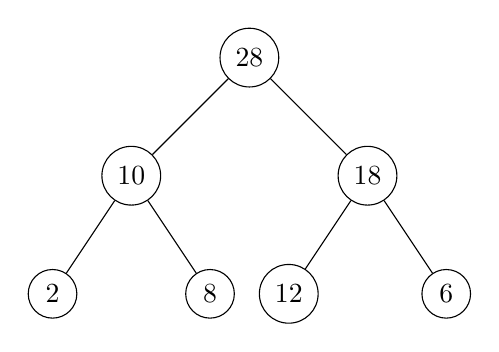
\begin{tikzpicture}[main/.style = {draw, circle}]
    % Nivel 1
    \node[main] (1) at (0,0) {28};

    % Nivel 2
    \node[main] (2) at (-1.5,-1.5) {10};
    \node[main] (3) at (1.5,-1.5) {18};

    % Nivel 3
    \node[main] (4) at (-2.5,-3) {2};
    \node[main] (5) at (-0.5,-3) {8};
    \node[main] (6) at (0.5,-3) {12};
    \node[main] (7) at (2.5,-3) {6};

    % Conexiones
    \draw (1) -- (2);
    \draw (1) -- (3);
    \draw (2) -- (4);
    \draw (2) -- (5);
    \draw (3) -- (6);
    \draw (3) -- (7);
\end{tikzpicture}

\lstinputlisting[language=C++]{secciones/estructuras/segment-tree.cpp}
\subsection{Array}
\lstinputlisting[language=C++]{secciones/estructuras/array.cpp}
\subsection{BitSet}
\begin{center}
    \begin{tabular}{||l|l|l||}
    \hline
    \textbf{Función}    & \textbf{Explicación}          & \textbf{O} \\ \hline

    \textbf{Template parameters} & & \\ \hline
        N               & número de bits             & O(1) \\ \hline

    \textbf{Member functions} & & \\ \hline
    (constructor) & construye el `bitset` & O(N) \\ \hline

    \textbf{Element access} & & \\ \hline
    operator[]          & accede a un bit específico    & O(1) \\ \hline
    all, any, none      & todos, algún o ningún bit está en true  & O(N) \\ \hline
    count               & número de bits establecidos en true     & O(N) \\ \hline
    size                & número de bits que contiene & O(1) \\ \hline

    \textbf{Modifiers} & & \\ \hline
        operator\&=  & & \\
        operator|= & & \\
        operator\textasciicircum= & & \\
        operator\textasciitilde= & & \\
        operator<<= & & \\
        operator>>= & & \\
        operator<< & & \\
        operator>> & & O(N) \\ \hline
        set() & pone todos los bits en el valor dado        & O(N) \\
        set(int pos) &                                      & O(1) \\ \hline
        reset() & establece bits en `false`                 & O(N) \\
        reset(int pos) &                                    & O(1) \\ \hline
        flip() & alterna los valores de los bits            & O(N) \\
        flip(int pos) & &O(1) \\ \hline

    \textbf{Conversions} & & \\ \hline
    to\_string & representación en cadena
    \end{tabular}
\end{center}

\newpage

\newpage
\section{Grafos}

\subsection{Recorrer Grafos}
Dado un Grafo como lista de adjacencias

\begin{lstlisting}[language=C++]
#include <bits/stdc++.h>
#define MAXN 100000
using namespace std;

vector<int> G[MAXN];
bool visited[MAXN];
\end{lstlisting}

Podemos recorrerlo con DFS o con BFS.

\subsubsection{DFS}
\lstinputlisting[language=C++]{secciones/grafos/dfs.cpp}

\subsubsection{BFS}
\lstinputlisting[language=C++]{secciones/grafos/bfs.cpp}
\newpage

\subsection{Camino Mínimo}

\subsubsection{Bellman-Ford}
El algoritmo de Bellman-Ford encuentra el camino desde un nodo de origen a todos los nodos del grafo. \\
\textbf{Complejidad = O(nm)}

\lstinputlisting[language=C++]{secciones/grafos/bellman-ford.cpp}
\subsubsection{Ciclos negativos}
El algoritmo es capaz de detectar ciclos negativos. Para eso Se debe correr una vez m'as
\newpage

\subsubsection{Dijkstra}
El algorimo necesita que todos los pesos sean > 0 \\
\textbf{Complejidad = O(n + m log m)}
\lstinputlisting[language=C++]{secciones/grafos/dijkstra.cpp}
\newpage
\subsubsection{Floyd-Warshall}
\lstinputlisting[language=C++]{secciones/grafos/floyd.cpp}

\newpage

\section{Strings}

\subsection{Hash}
\lstinputlisting[language=C++]{secciones/strings/hash.cpp}

\newpage

\newpage
\section{Geometria}

\subsection{Punto}
\lstinputlisting[language=C++]{secciones/geometria/pto.cpp}

\subsection{Line}
\lstinputlisting[language=C++]{secciones/geometria/line.cpp}

\subsection{Segment}
\lstinputlisting[language=C++]{secciones/geometria/segment.cpp}

\subsection{Circle}
\lstinputlisting[language=C++]{secciones/geometria/circle.cpp}

\newpage

\section{DP}
\subsection{Game}
\lstinputlisting[language=C++]{secciones/dp/juegos.cpp}

\subsection{Long common subsecuence}
\lstinputlisting[language=C++]{secciones/dp/lcs.cpp}

\subsection{Matching mask}
\lstinputlisting[language=C++]{secciones/dp/mask.cpp}

\subsection{DP rangos}
\lstinputlisting[language=C++]{secciones/dp/rangos.cpp}

\newpage

\section{Utils}

\subsection{Binary Search}
\lstinputlisting[language=C++]{secciones/utils/bs.cpp}

\subsection{Sort}
Ordenar un vector de pair por su segunda componente
\begin{lstlisting}[language=C++]
vector<pair<int, int>> v;

bool sortbysec(const pair<int,int> &a, const pair<int,int> &b){
	return (a.second < b.second);
}

sort(v.begin(), v.end(), sortbysec);
\end{lstlisting}
\subsection{Cout para doubles}
\begin{lstlisting}[language=C++]
cout << fixed << setprecision(20) << ans << endl;
\end{lstlisting}
\subsection{Prev permutation}
\lstinputlisting[language=C++]{secciones/utils/prevpermutation.cpp}
\subsection{MO}
\lstinputlisting[language=C++]{secciones/utils/mo.cpp}

\subsection{Criba}
Nros primos hasta maxp
\lstinputlisting[language=C++]{secciones/utils/criba.cpp}

\subsection{Subconjuntos}
Subconjuntos distintos de un conjunto
\lstinputlisting[language=C++]{secciones/utils/Subconjuntos.cpp}

\subsection{Propiedades del Bitwise XOR ($\oplus$)}
\begin{enumerate}
    \item \textbf{Identidad:} 
    \[
    a \oplus 0 = a
    \]

    \item \textbf{Autoinversión:} 
    \[
    a \oplus a = 0
    \]

    \item \textbf{Conmutativa:} 
    \[
    a \oplus b = b \oplus a
    \]

    \item \textbf{Asociativa:} 
    \[
    (a \oplus b) \oplus c = a \oplus (b \oplus c)
    \]

    \item \textbf{Autoeliminación:} 
    \[
    a \oplus a \oplus b = 0 \oplus b = b
    \]

    \item \textbf{Uso práctico: Encontrar elemento único} \\
    Si todos los elementos de un conjunto aparecen dos veces excepto uno:
    \[
    x_1 \oplus x_2 \oplus \dots \oplus x_n = \text{elemento único}
    \]
\end{enumerate}

\newpage





\end{document}
